\documentclass[10pt,xcolor=dvipsnames]{beamer}
\usetheme[progressbar=frametitle]{metropolis}
%\usepackage[usenames,dvipsnames]{xcolor}
%\usepackage{appendixnumberbeamer}
\usepackage{booktabs}
\usepackage{color}
\usepackage[scale=2]{ccicons}

\usepackage{pgfplots}
\usepgfplotslibrary{dateplot}

\usepackage{xspace}
\newcommand{\themename}{\textbf{\textsc{metropolis}}\xspace}
\definecolor{maroon}{RGB}{175,50,53} % Define a custom maroon color

\usepackage{pdfpages}
\setbeamercolor{section title}{fg=maroon,bg=maroon}
\setbeamercolor*{structure}{bg=maroon!20,fg=maroon}
\setbeamercolor*{palette primary}{use=structure,fg=white,bg=structure.fg}
\setbeamercolor{progress bar}{fg=gray, bg=gray}

%%%%%%%%%%%%%%%%%%%%%%%%%%%%%%%%%%%%%%%%%%%%%%%%%%%%%%%%%%%%%%%%%%%%%

\title{My Progress}
\subtitle{MonoHiggs Group presentation}
\date{\today}
\author{Prayag Yadav}
\institute{University of Hyderabad}
\titlegraphic{\hfill
\includegraphics[height=1.5cm]{uoh_logo.jpg}}

%%%%%%%%%%%%%%%%%%%%%%%%%%%%%%%%%%%%%%%%%%%%%%%%%%%%%%%%%%%%%%%%%%%%%

\begin{document}

\maketitle

\begin{frame}{Table of contents}
  \setbeamertemplate{section in toc}[sections numbered]
  \tableofcontents%[hideallsubsections]
\end{frame}

\section[Basic kinematic plots without selections, corrections and Scale Factors ]{Basic kinematic plots }

\begin{frame}[fragile]{BTag Scores : MC }
\begin{figure}
  \centering
  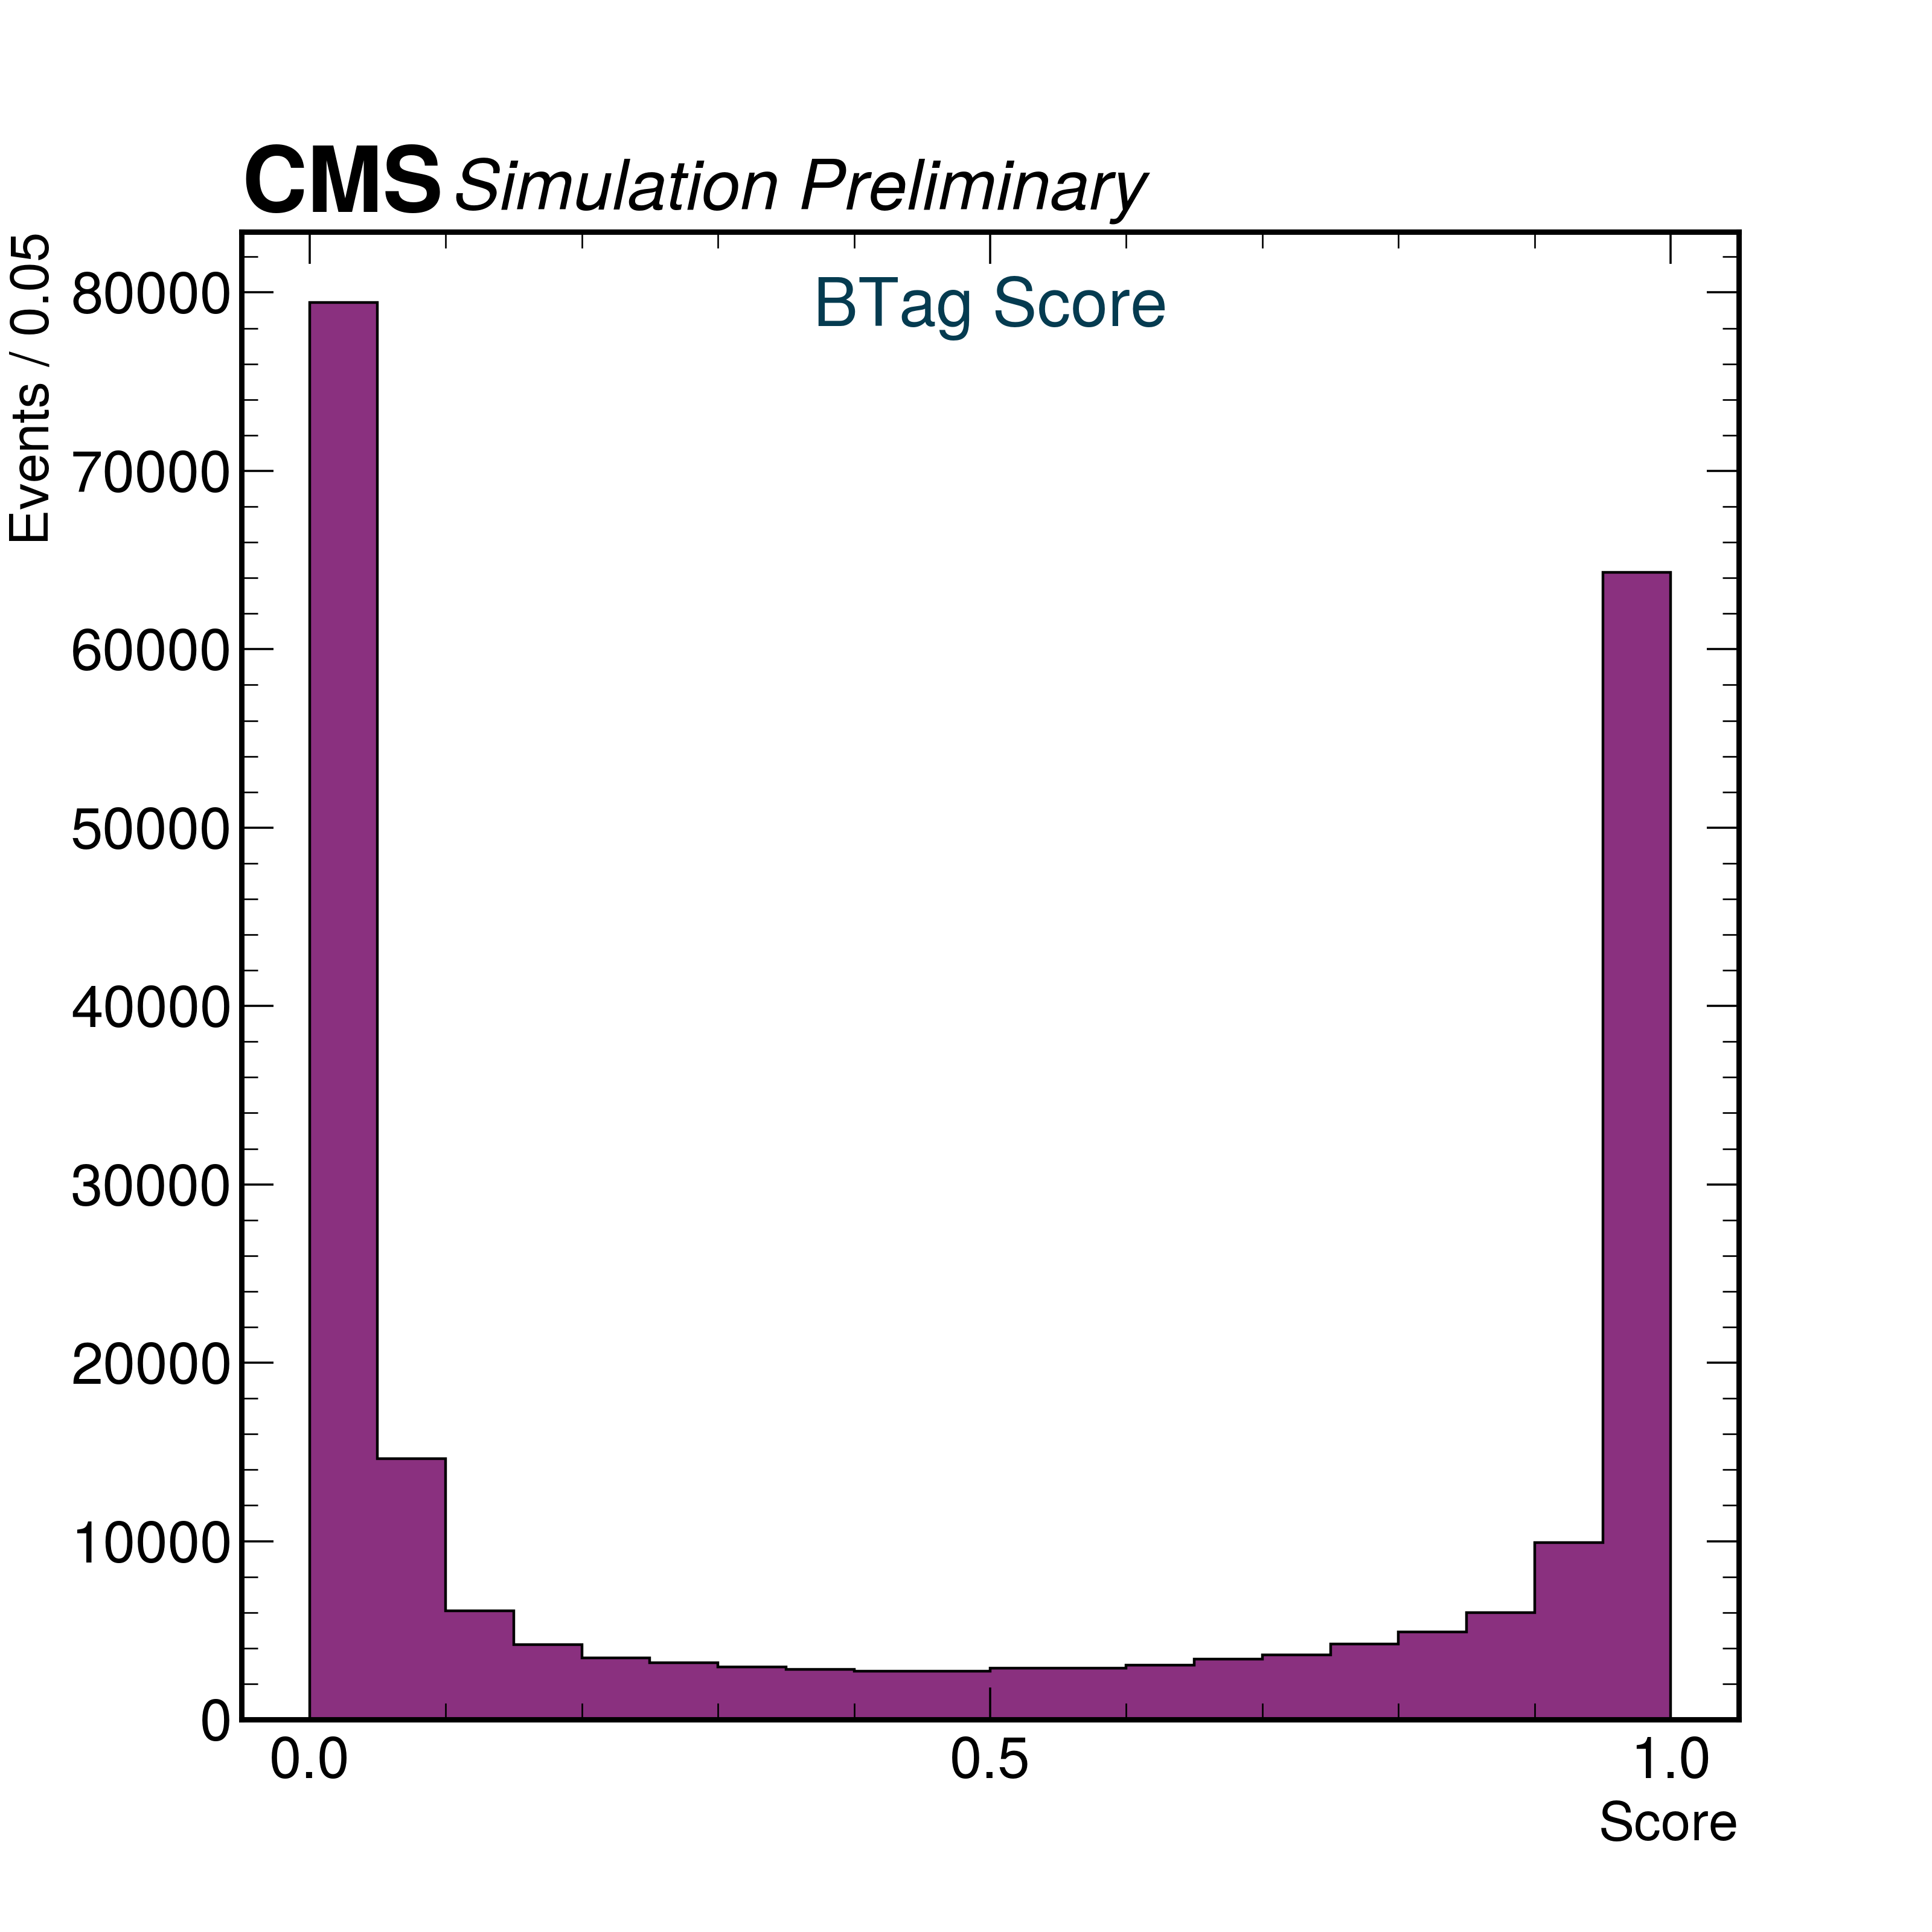
\includegraphics[width=0.65\textwidth]{../Kinematics/TagMC.png}
  \label{TagMC}
  \caption{BTag score for signal MC sample}
\end{figure}  
\end{frame}

\begin{frame}[fragile]{BTag Scores : Data}

  \begin{figure}
    \centering
    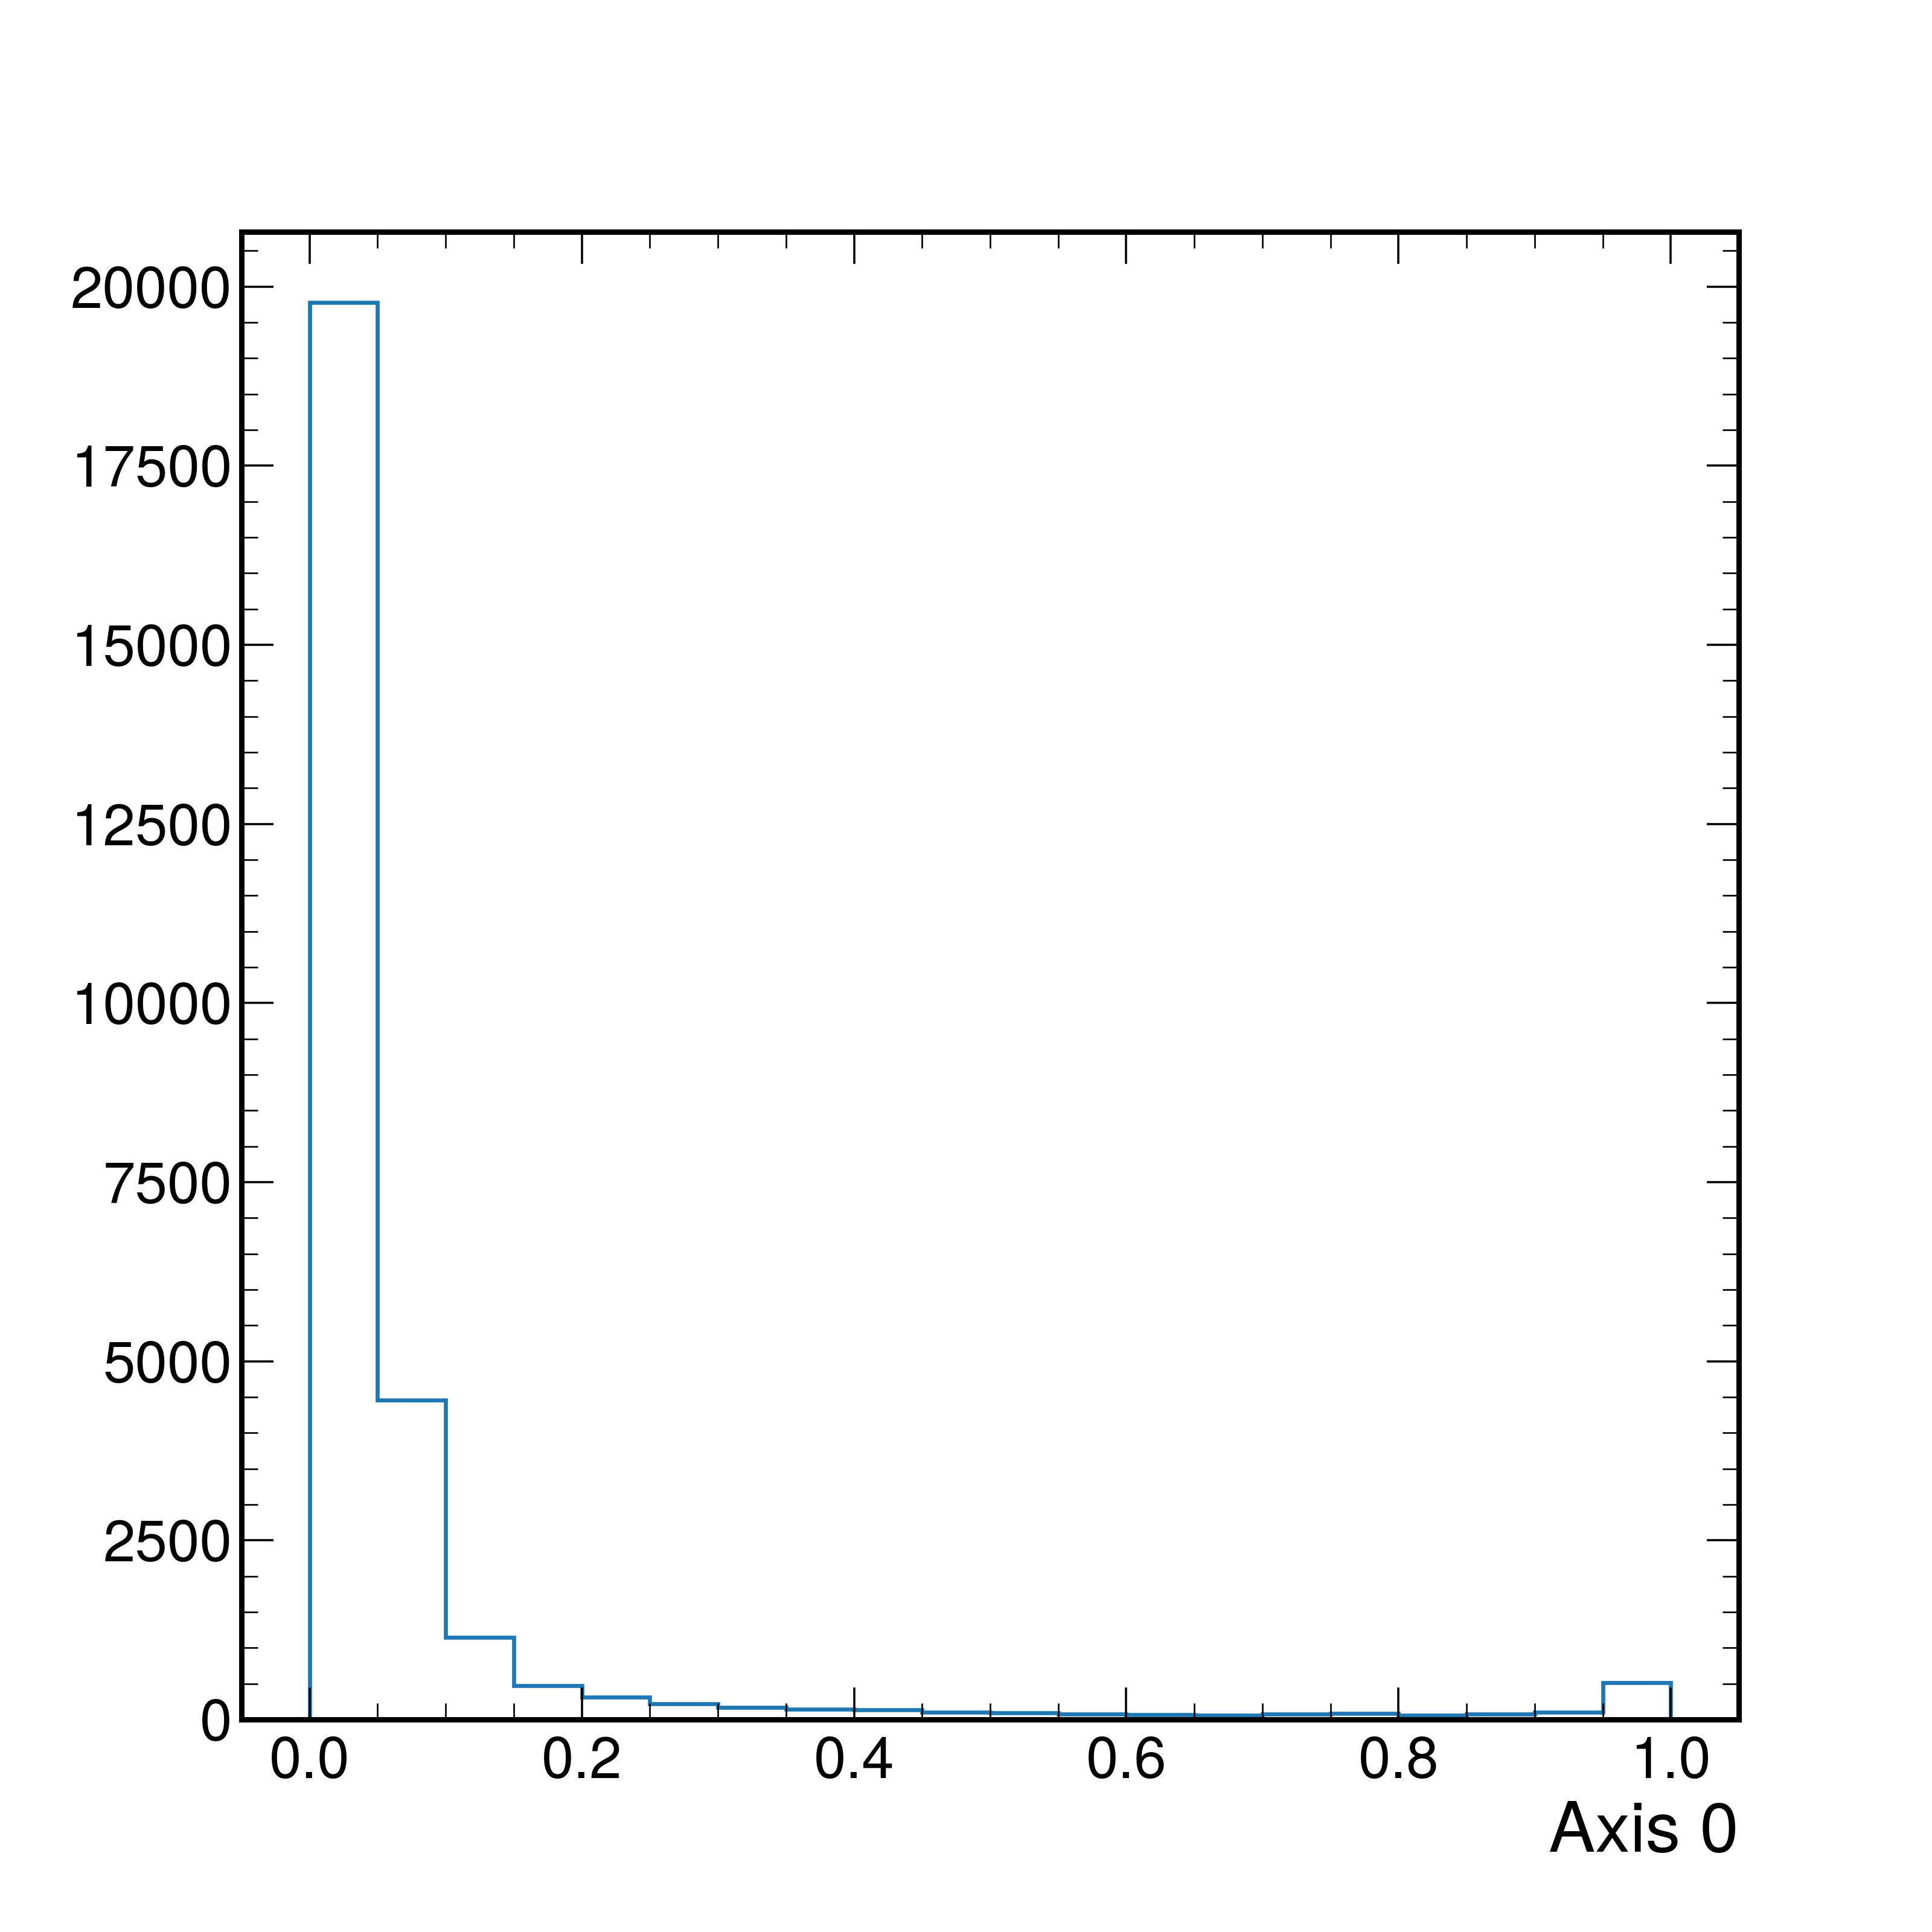
\includegraphics[width=0.65\textwidth]{../Kinematics/TagData.png}
    \label{TagData}
    \caption{BTag score for Data samples}
  \end{figure}  

\end{frame}

\begin{frame}[fragile]{Jet $p_t$ : MC }
  \begin{figure}
    \centering
    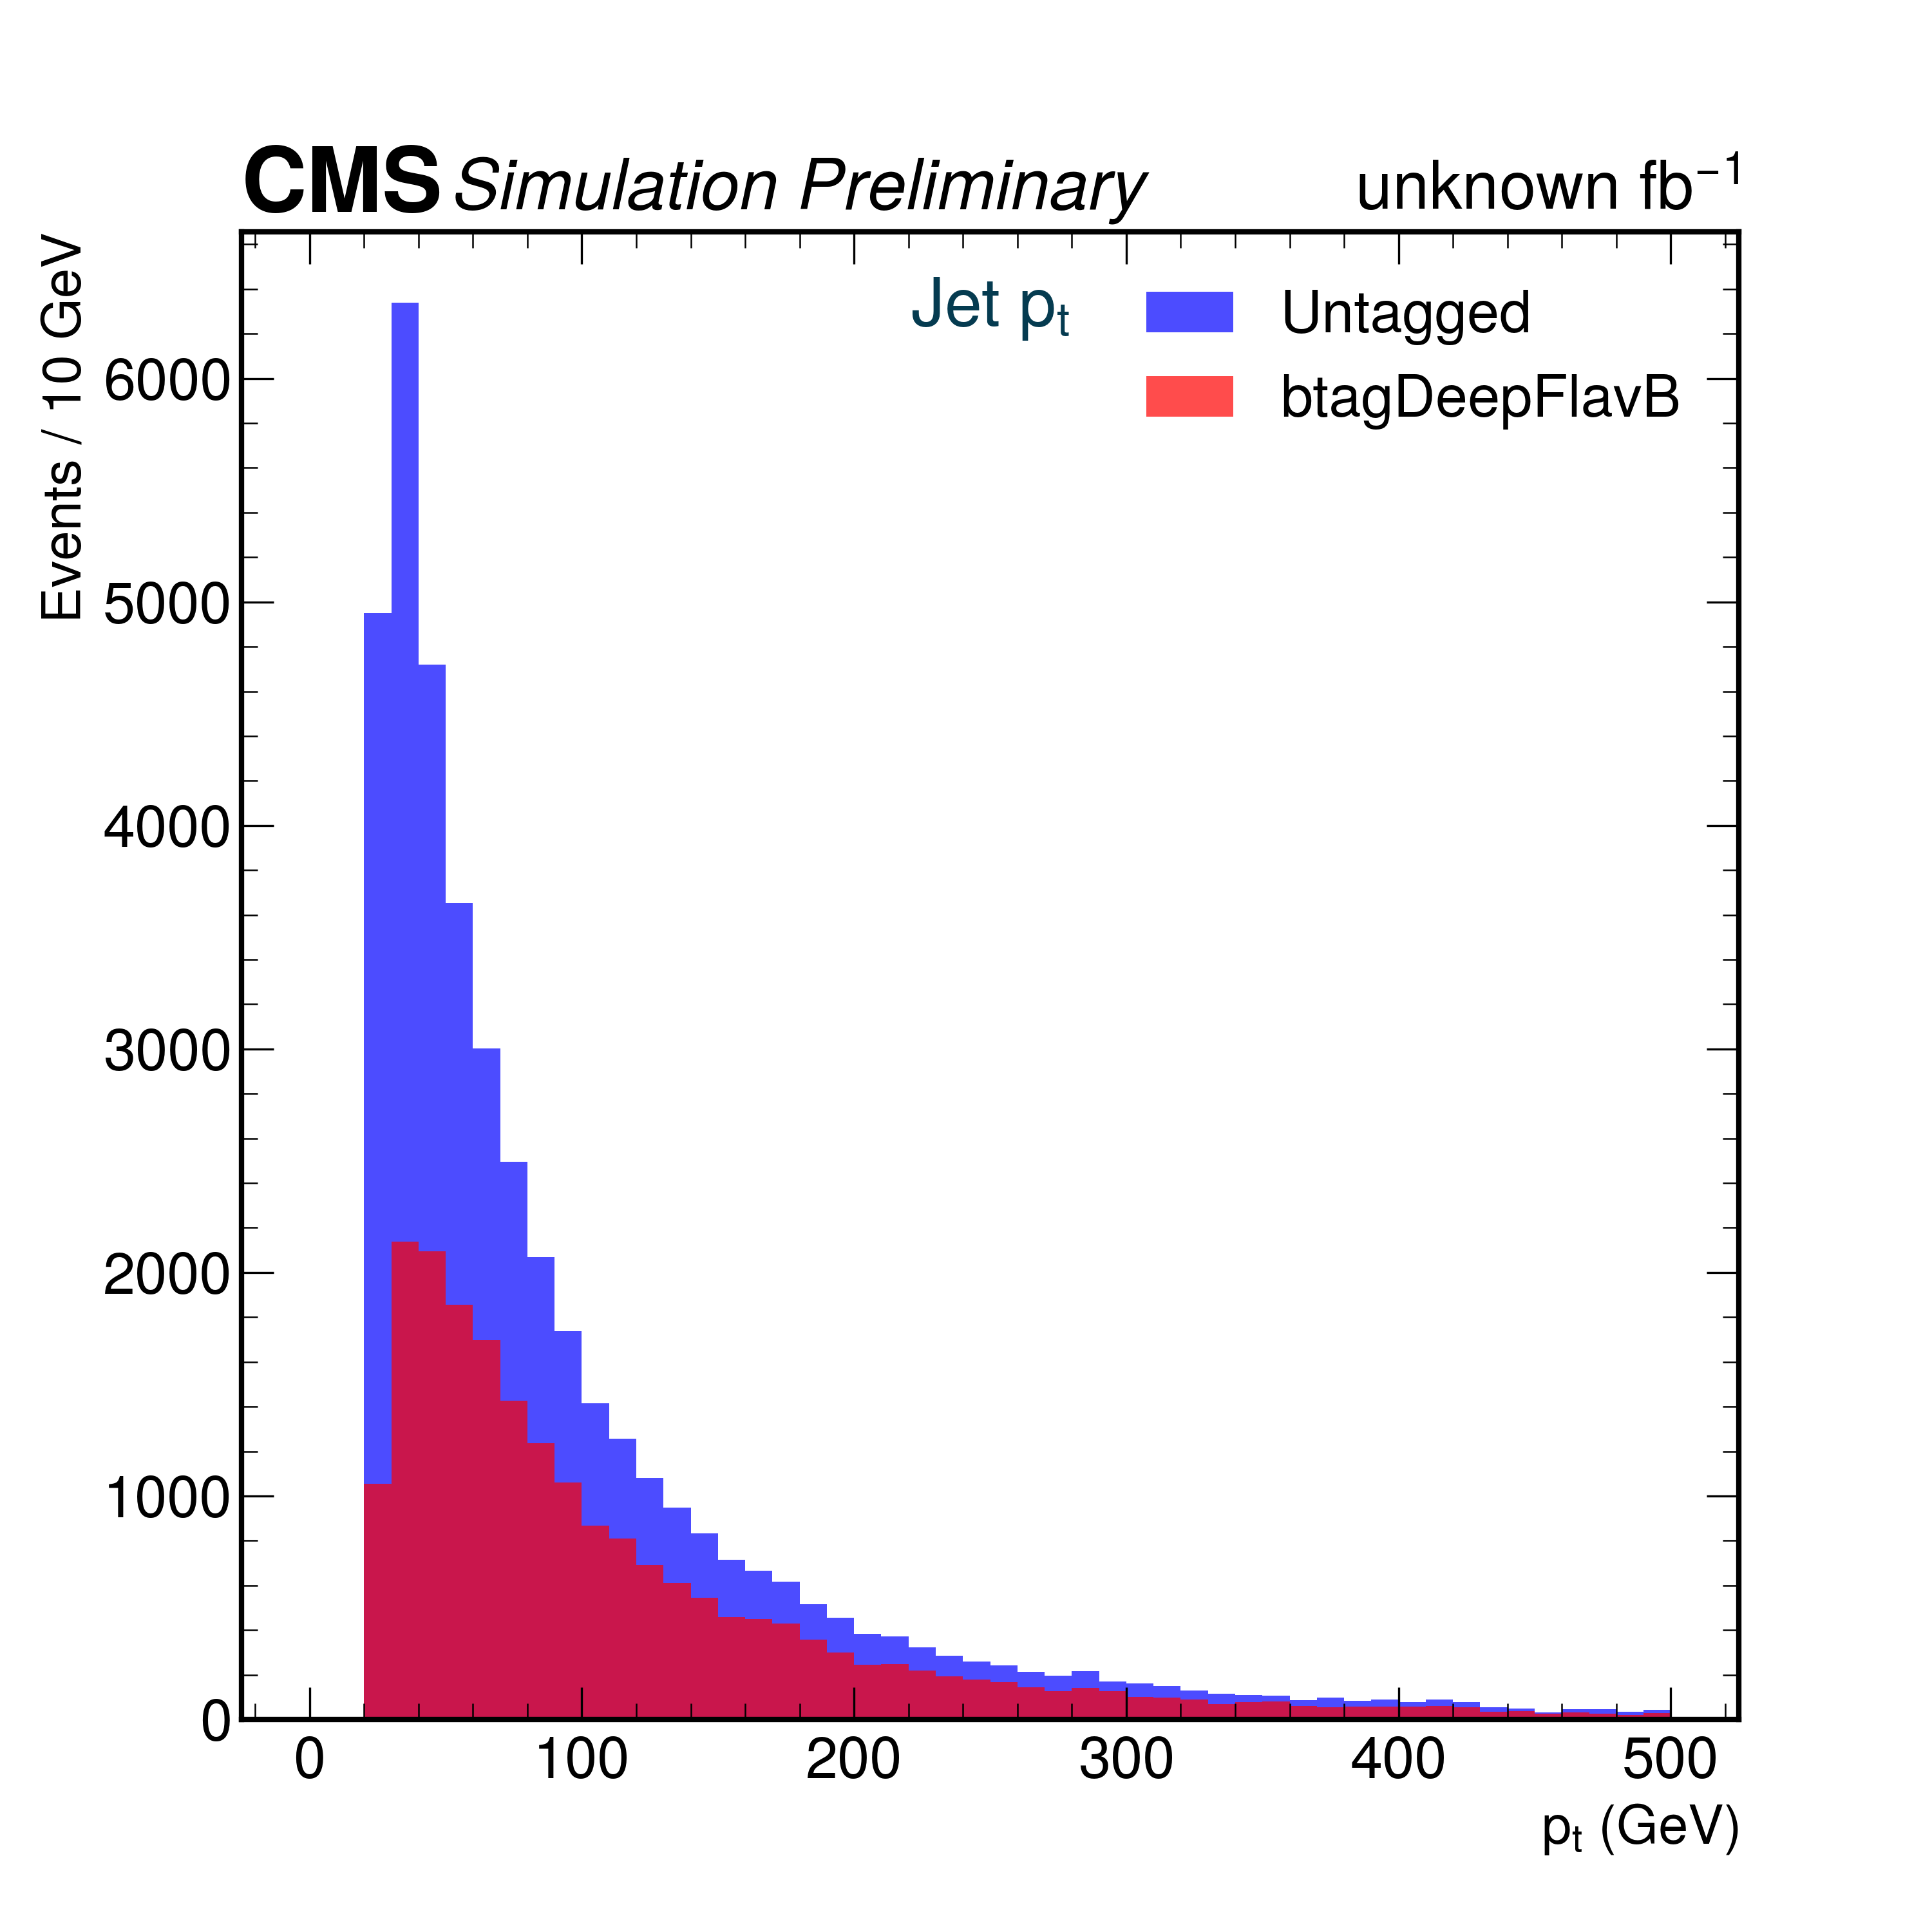
\includegraphics[width=0.65\textwidth]{../Kinematics/JetsMC.png}
    \label{JetMC}
    \caption{Jet $p_t$ of signal MC samples}
  \end{figure}  
  \end{frame}
  
  \begin{frame}[fragile]{Jet $p_t$ : Data}
  
    \begin{figure}
      \centering
      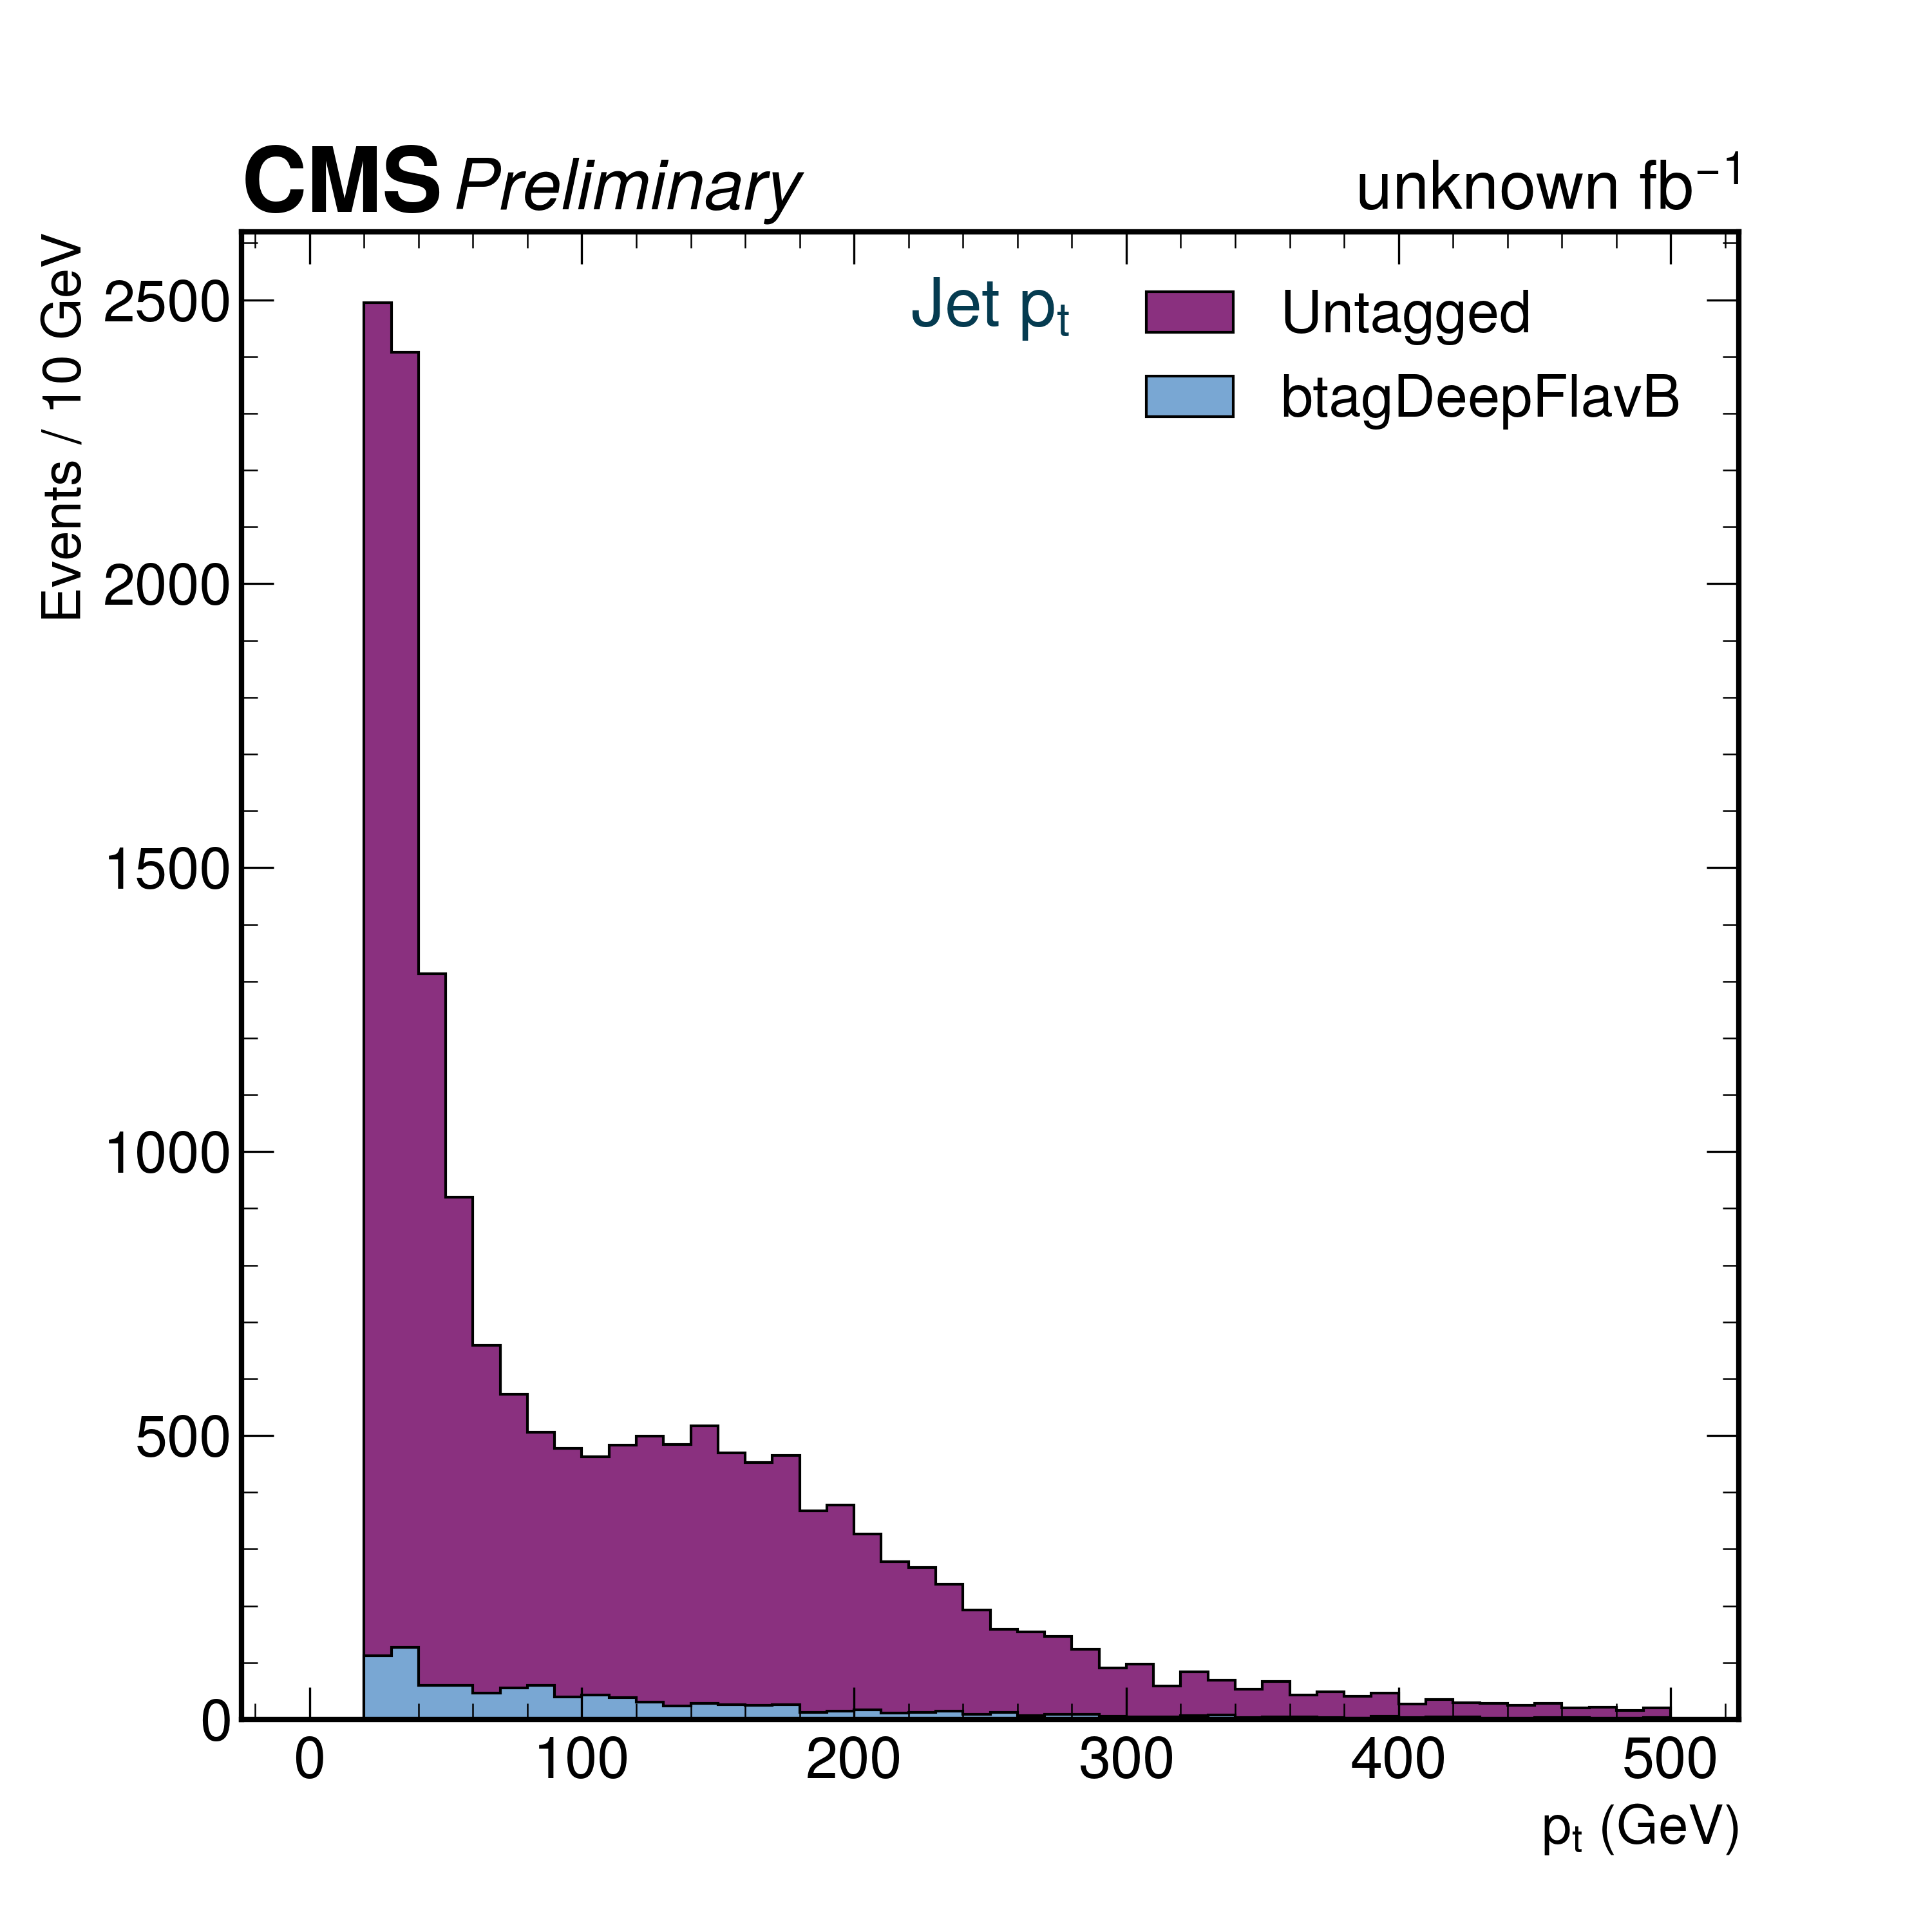
\includegraphics[width=0.65\textwidth]{../Kinematics/JetsData.png}
      \label{JetData}
      \caption{Jet $p_t$ of Data samples}
    \end{figure}  
  
  \end{frame}

  \begin{frame}[fragile]{DiJet mass : MC }
    \begin{figure}
      \centering
      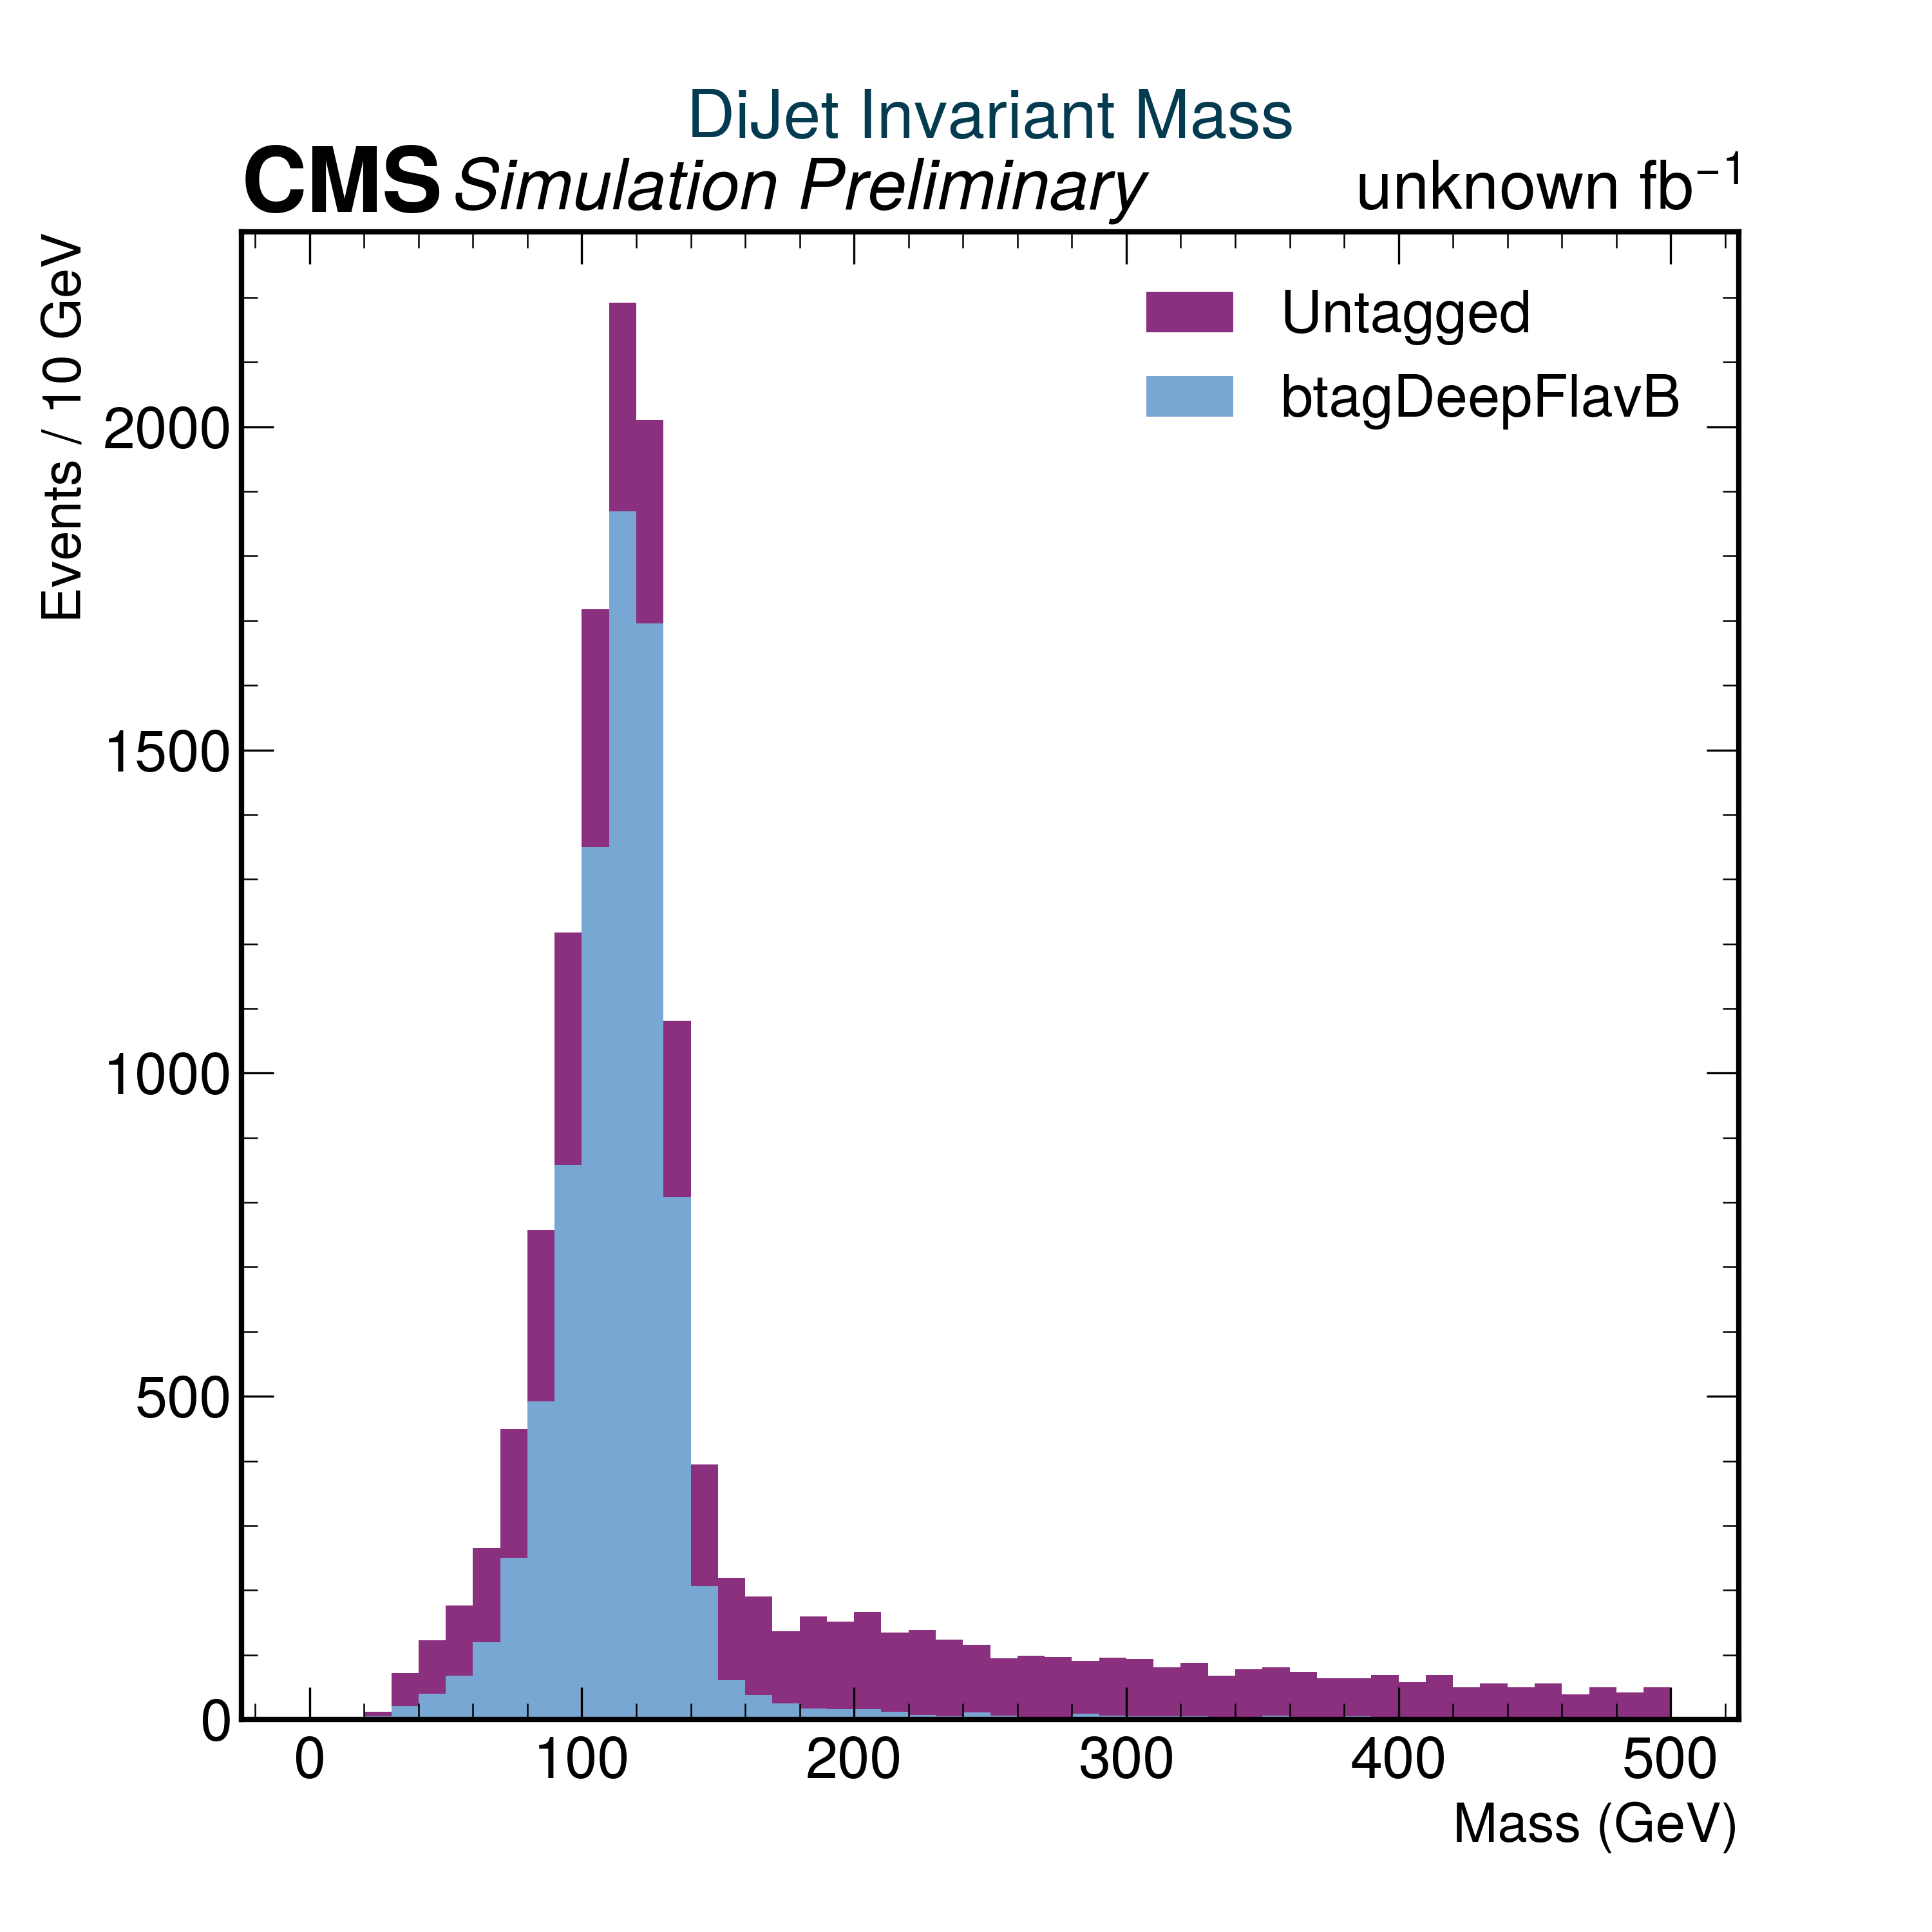
\includegraphics[width=0.65\textwidth]{../Kinematics/DiJetsMC.png}
      \label{DiJetMC}
      \caption{DiJet mass of signal MC samples}
    \end{figure}  
  \end{frame}

  \begin{frame}[fragile]{DiJet mass : Data }
    \begin{figure}
      \centering
      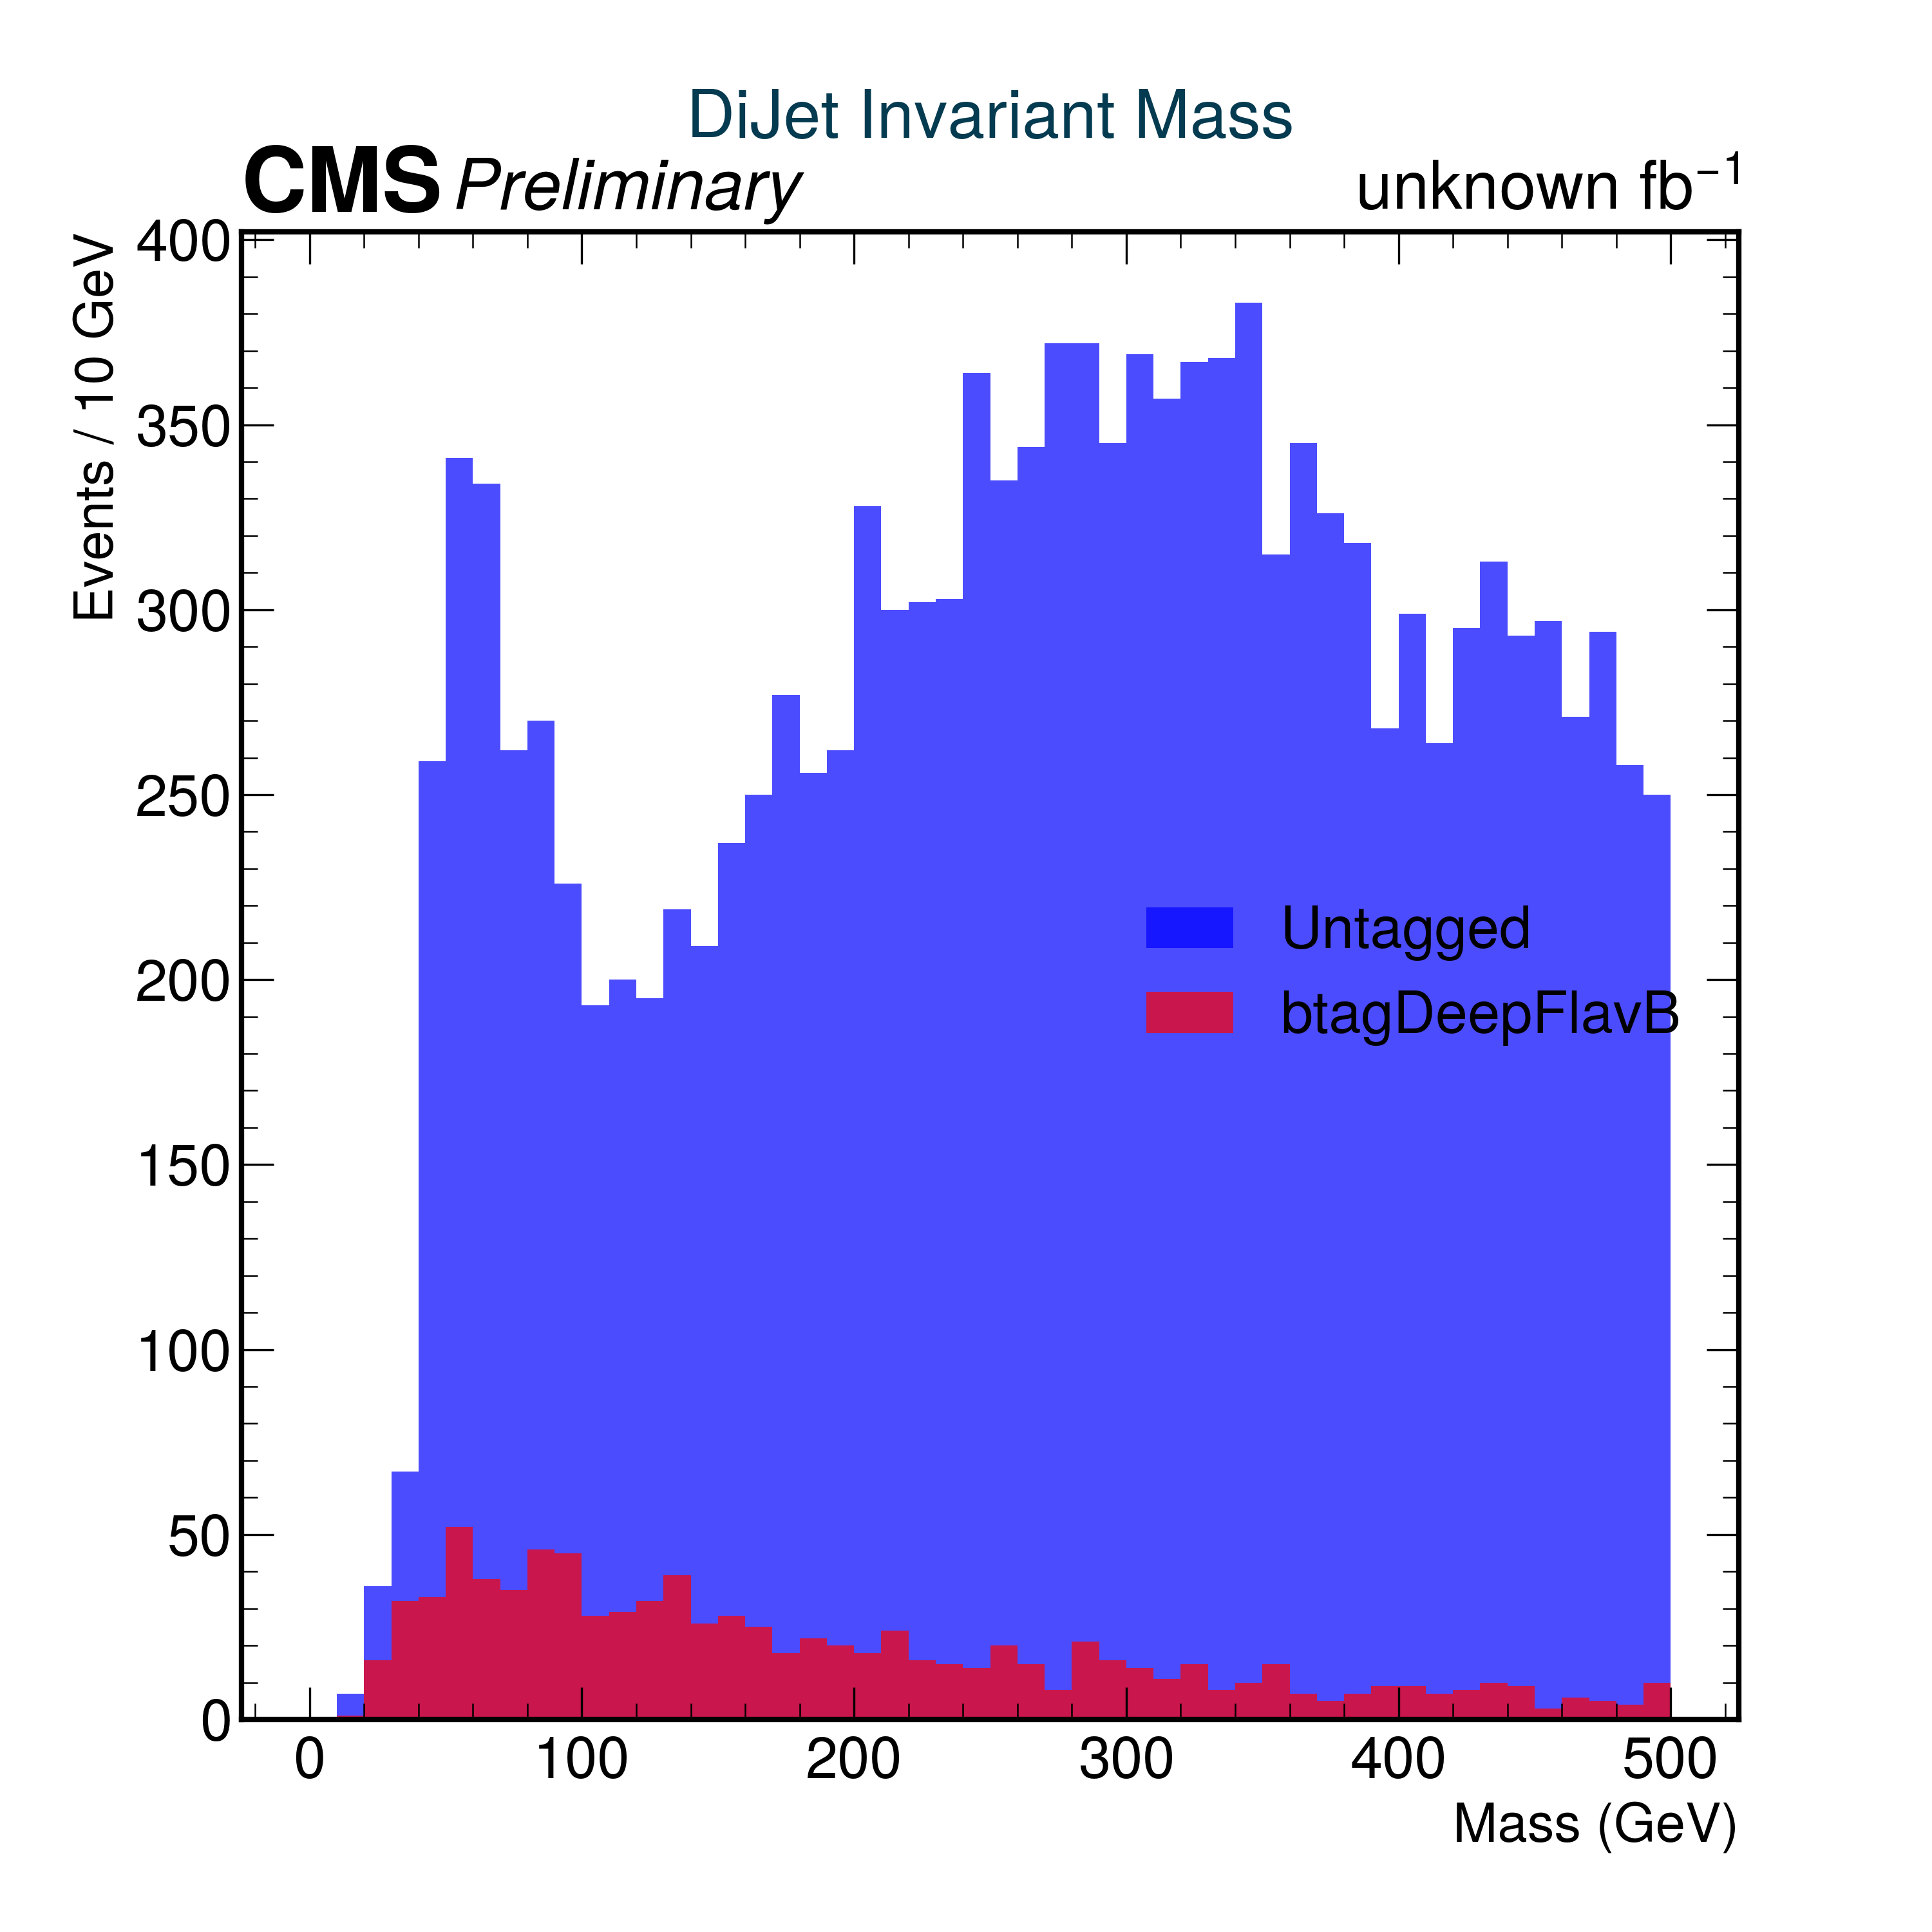
\includegraphics[width=0.65\textwidth]{../Kinematics/DiJetsData.png}
      \label{DiJetsData}
      \caption{DiJet mass of Data samples}
    \end{figure}  
  \end{frame}

\appendix

% \begin{frame}[fragile]{Backup slides}

% \end{frame}

\begin{frame}[allowframebreaks]{References}

  \bibliography{references}
  \bibliographystyle{abbrv}

\end{frame}

\end{document}
